\documentclass[11pt,a4paper]{article}
\usepackage[utf8]{inputenc}
\usepackage[T1]{fontenc}
\usepackage{lmodern}
\usepackage{xcolor}
\renewcommand{\contentsname}{Spis treści}
\renewcommand{\tablename}{Tabela}
\renewcommand{\figurename}{Rys.}
\hyphenpenalty=3000 \tolerance=2000 \emergencystretch=2em
\usepackage[margin=2.0cm]{geometry}
\usepackage{tikz}
\usepackage{booktabs}
\usepackage{longtable}
\usepackage{enumitem}
\usepackage{titlesec}
\usepackage{parskip}
\usepackage[colorlinks=true,linkcolor=blue!50!black]{hyperref}
\titleformat{\section}{\large\bfseries}{\thesection.}{0.6em}{}
\titleformat{\subsection}{\normalsize\bfseries}{\thesubsection.}{0.6em}{}
\setlist{nosep,leftmargin=1.4em}
\newcommand{\ohm}{$\Omega$}
\newcommand{\stC}{$^\circ$C}

\title{\textbf{AMPERE POINT}\\[4pt]
\large Instalacje elektryczne a ładowanie EV --- kompletny przewodnik\\[2pt]
\normalsize wymagania, różnice między instalacjami w Polsce i ich wpływ na problemy z ładowaniem\\
wersja 1}
\author{Opracowanie wewnętrzne AMPERE POINT}
\date{10 lipca 2026}

\begin{document}
\maketitle
\vspace{-1.4em}

\noindent\textbf{Dla kogo i po co.} Ten przewodnik jest dla osoby bez doświadczenia z instalacjami
elektrycznymi (wystarczą podstawy elektrotechniki: prawo Ohma, moc, prąd przemienny). Cel praktyczny:
duża część ,,usterek'' ładowarek to w rzeczywistości \textbf{wady instalacji klienta} --- ładowarka
wraca do serwisu, na stole działa bez zarzutu, a u klienta problem wraca. Żeby takie przypadki
rozpoznawać przez telefon (konkretnymi pytaniami) i odtwarzać na stanowisku, trzeba rozumieć:
czego ładowanie EV wymaga od instalacji, czym różnią się instalacje spotykane w Polsce i ---
najważniejsze --- \textbf{jakie wady instalacji nie przeszkadzają zwykłym urządzeniom, a ładowanie
psują}. Rysunki w dokumencie są schematyczne (własne), rysowane pod zrozumienie, nie pod normę.

\tableofcontents

\section{Dlaczego ładowanie EV to najtrudniejszy odbiornik w domu}
\label{sec:dlaczego}
Wszystkie problemy z tego przewodnika mają wspólny korzeń: \textbf{ładowarka EV obciąża instalację
inaczej niż cokolwiek, co klient zna}. Cztery różnice:

\textbf{1. Prąd ciągły przez wiele godzin.} Czajnik pobiera 10~A przez 3 minuty, piekarnik grzeje
z przerwami (termostat), pralka tylko chwilami. Ładowarka pobiera 10--32~A \textbf{bez przerwy przez
4--10 godzin}. Ciepło wydzielane na każdej niedoskonałości połączenia rośnie z kwadratem prądu
($P=I^2R$) i --- co kluczowe --- \textbf{z czasem}: słaby styk przy czajniku nie zdąży się nagrzać,
przy ładowaniu nocnym osiąga temperaturę równowagi, której tworzywa nie wytrzymują. Dlatego wada,
która ,,nie istnieje'' dla AGD, przy EV topi gniazdo.

\textbf{2. Ładowarka sprawdza instalację.} Zwykłe urządzenie nie wie nic o instalacji --- grzeje,
kręci, świeci. Ładowarka (dla bezpieczeństwa użytkownika) \textbf{aktywnie kontroluje}: obecność
i jakość uziemienia PE, poprawność L--N (zamiana blokuje pracę), napięcie w dopuszczalnym oknie,
prąd upływu (własny czujnik 30~mA AC $+$ 6~mA DC). Instalacja z wadą, której nikt nigdy nie widział,
nagle ,,nie działa'' --- bo pierwszy raz coś ją naprawdę sprawdziło.

\textbf{3. Praca na granicy obwodu.} Ładowanie ustawia się zwykle na maksimum tego, co obwód
teoretycznie daje (16~A z gniazda 16~A). Zapas, który maskuje wady przy mniejszych prądach, znika.

\textbf{4. Współpraca trzech stron.} W torze są: instalacja, ładowarka i \textbf{samochód} (to on
prostuje prąd i decyduje, ile pobiera). Auto też pilnuje napięcia i jakości zasilania --- potrafi
samo zredukować prąd albo przerwać, co klient widzi jako ,,wolno ładuje/przerywa'', choć ładowarka
jest sprawna.

\begin{longtable}{@{}p{0.24\textwidth}p{0.16\textwidth}p{0.16\textwidth}p{0.34\textwidth}@{}}
\toprule
\textbf{Odbiornik} & \textbf{Prąd} & \textbf{Czas pracy} & \textbf{Czego wymaga od instalacji}\\
\midrule
czajnik & 8--10 A & minuty & niczego nie sprawdza; krótki impuls ciepła\\
pralka / zmywarka & szczytowo 10 A & grzanie: kilkanaście minut & niczego nie sprawdza\\
piekarnik & 10--14 A & z przerwami (termostat) & obwód dedykowany zwykle jest\\
indukcja & do 16--32 A & krótkie szczyty & jw.\\
\textbf{ładowarka EV} & \textbf{10--32 A} & \textbf{4--10 h bez przerwy} & sprawdza PE, L--N, napięcie, upływ; grzeje każdy słaby punkt do równowagi termicznej\\
\bottomrule
\end{longtable}

\section{Elementarz: jak zbudowana jest instalacja domowa}
\label{sec:elementarz}
Droga prądu: stacja transformatorowa $\to$ linia (kablowa w ziemi albo napowietrzna na słupach)
$\to$ \textbf{złącze} budynku $\to$ licznik $\to$ \textbf{rozdzielnica} (,,skrzynka z bezpiecznikami'')
$\to$ obwody w ścianach $\to$ gniazda. Po drodze każdy element ma rezystancję i każdy bywa słabym
punktem.

\subsection{Zabezpieczenie nadprądowe (,,eska'', np. B16)}
Wyłącznik instalacyjny chroni \textbf{przewody} (nie urządzenia!) przed przeciążeniem i zwarciem.
Oznaczenie ,,B16'': charakterystyka B (wyzwala zwarciowo przy 3--5$\times$ prądu znamionowego),
16~A prądu znamionowego. Ważne dla EV: B16 \textbf{nie wyłączy się} od 16~A --- przewód i gniazdo
muszą ten prąd znosić godzinami; wyłączy się dopiero przy wyraźnym przeciążeniu (np. 20~A po
kilkudziesięciu minutach) albo zwarciu. W starych instalacjach zamiast wyłączników bywają
\textbf{bezpieczniki topikowe} (,,korki'') --- działają, ale bywają ,,naprawiane'' drutem
(śmiertelnie niebezpieczna praktyka) i nie mają charakterystyki dobranej do EV.

\subsection{Wyłącznik różnicowoprądowy (RCD, ,,różnicówka'')}
RCD porównuje prąd wypływający przewodem L z wracającym przewodem N. Różnica oznacza, że część
prądu ucieka inną drogą --- przez uszkodzoną izolację, wodę, człowieka. Gdy różnica przekroczy
próg (w mieszkaniach 30~mA), RCD wyłącza obwód w ułamku sekundy. Dwie rzeczy, które trzeba
zrozumieć przy EV:
\begin{itemize}
\item \textbf{RCD sumuje upływy całego chronionego obszaru.} Każde urządzenie z filtrem
przeciwzakłóceniowym (pralka, komputer, indukcja) ,,upuszcza'' legalnie 0,5--2~mA do PE. Ładowarka
z autem dokłada swoje kilka mA. Jeśli jeden RCD chroni pół mieszkania, suma potrafi podejść pod
próg --- i wtedy \emph{cokolwiek} (wilgotna noc, lodówka) przelewa czarę: RCD ,,wyzwala losowo''.
\item \textbf{RCD ma typ --- i to jest kluczowe dla EV} (rys.~\ref{fig:rcd}). Typ \textbf{AC}
widzi tylko upływ sinusoidalny; typ \textbf{A} także pulsujący (wyprostowany); typ \textbf{B}
również \textbf{gładki prąd stały}. Elektronika mocy auta może w razie awarii wypuścić upływ
\emph{stały} --- a gładki prąd stały potrafi \textbf{oślepić} RCD typu AC/A (podmagnesowuje rdzeń
przekładnika: różnicówka przestaje widzieć również zwykłe upływy!). Dlatego norma wymaga dla EV:
RCD typu B \emph{albo} RCD typu A $+$ układ \textbf{RDC-DD} wykrywający 6~mA DC --- i dokładnie
ten układ (typ A 30~mA $+$ 6~mA DC) mają w środku ładowarki AMPERE POINT. W starych instalacjach
w Polsce dominują RCD typu AC --- patrz rozdz.~\ref{sec:niekrytyczne}.
\end{itemize}

\begin{figure}[h]
\centering
\begin{tikzpicture}[x=1cm,y=1cm,scale=0.9]
\foreach \ox/\tit/\wid in {0/{upływ sinusoidalny}/{AC, A, F, B}, 4.4/{pulsujący (wyprostowany)}/{A, F, B}, 8.8/{gładki DC (np. 6 mA)}/{tylko B / RDC-DD}, 13.2/{wysokie częstotliwości}/{F, B}}{
  \draw[->] (\ox,0) -- (\ox+3.4,0);
  \draw[->] (\ox,-0.9) -- (\ox,1.1);
  \node[font=\scriptsize, align=center] at (\ox+1.7,1.5) {\tit};
  \node[font=\scriptsize\bfseries] at (\ox+1.7,-1.35) {widzi: \wid};}
\draw[thick] plot[domain=0:3.2,samples=60] (\x,{0.7*sin(2.2*\x r)});
\draw[thick] plot[domain=4.4:7.6,samples=80] (\x,{0.7*abs(sin(2.2*(\x-4.4) r))});
\draw[thick] (8.8,0.55) -- (12.0,0.55);
\draw[thick] plot[domain=13.2:16.4,samples=160] (\x,{0.55*sin(9*(\x-13.2) r)});
\end{tikzpicture}
\caption{Cztery rodzaje prądu upływu i typy RCD, które je wykrywają. Stary RCD ,,AC'' nie widzi
dwóch prawych przebiegów --- a gładki DC dodatkowo go oślepia.}
\label{fig:rcd}
\end{figure}

\subsection{Przewody i połączenia}
Miedź (Cu) albo --- w instalacjach z lat 60.--80. --- \textbf{aluminium} (Al). Przekrój podaje się
w mm$^2$: typowo 1,5~mm$^2$ (oświetlenie), 2,5~mm$^2$ (gniazda). Rezystancja przewodu:
$R=\rho\cdot 2L/S$ (podwójna długość: prąd płynie tam i z powrotem), $\rho_{Cu}\approx0{,}0175$,
$\rho_{Al}\approx0{,}028$~\ohm$\cdot$mm$^2$/m. Każde \textbf{połączenie} (puszka, zacisk, gniazdo)
to dodatkowa rezystancja --- dobra: pojedyncze m\ohm; poluzowana lub skorodowana: dziesiąte części
\ohm{}, czyli przy 16~A dziesiątki watów ciepła w jednym punkcie. Aluminium ma dodatkową wadę:
\textbf{płynie} pod dociskiem i utlenia się --- zaciski luzują się \emph{same z czasem}, dlatego
usterka wraca po naprawie.

\subsection{Gniazdo Schuko i przewód PE}
Gniazdo ,,z bolcami'' (Schuko) trzyma wtyczkę sprężystymi stykami. Znamionowo 16~A --- ale norma
gniazd nie zakłada 16~A \textbf{ciągle przez godziny}; zużyte sprężyny (wielokrotne wtykanie,
tanie gniazdo, wcześniejsze przegrzania) podnoszą rezystancję styku wielokrotnie. Dlatego ładowarki
przenośne domyślnie ograniczają prąd z gniazda (seria B: wybór 8/10/13/16~A) --- i dlatego ,,grzanie
wtyczki'' jest najczęstszym objawem instalacyjnym (rozdz.~\ref{sec:niekrytyczne}).
\textbf{Przewód ochronny PE} (żółto-zielony) na co dzień \emph{nie przewodzi prądu} --- czeka na
awarię, żeby odprowadzić prąd zwarcia/upływu i pozwolić zabezpieczeniom zadziałać. Skutek:
\textbf{uszkodzony PE jest niewidoczny} --- wszystko działa latami, aż przyjdzie awaria (albo
ładowarka, która PE sprawdza od razu).

\section{Układy sieci spotykane w Polsce: TN-C, TN-C-S, TN-S, TT}
\label{sec:uklady}
,,Układ sieci'' opisuje, jak poprowadzone są przewód neutralny (N) i ochronny (PE) od transformatora
do gniazdka --- i to jest największa systemowa różnica między polskimi instalacjami
(rys.~\ref{fig:uklady}).

\begin{figure}[h]
\centering
\begin{tikzpicture}[x=1cm,y=1cm,scale=0.92,font=\scriptsize]
\newcommand{\uziom}[2]{\draw (#1,#2) -- (#1,#2-0.25) (#1-0.22,#2-0.25)--(#1+0.22,#2-0.25) (#1-0.14,#2-0.35)--(#1+0.14,#2-0.35) (#1-0.07,#2-0.45)--(#1+0.07,#2-0.45);}
\foreach \ox/\tit in {0/{TN-C (stara)}, 5.8/{TN-S (nowa)}, 11.6/{TT (częsta na wsi)}}{
  \draw (\ox+0.2,2.6) circle (0.35); \node at (\ox+0.2,2.6) {Tr};
  \node[font=\scriptsize\bfseries] at (\ox+2.3,3.4) {\tit};
  \draw[thick] (\ox+0.55,2.8) -- (\ox+4.6,2.8); \node[right] at (\ox+4.6,2.8) {L};
  \draw (\ox+3.4,1.0) rectangle (\ox+4.6,2.0); \node at (\ox+4.0,1.75) {odbiornik};
  \draw (\ox+4.0,2.8) -- (\ox+4.0,2.0);}
\draw[thick] (0.55,2.2) -- (4.6,2.2); \node[right] at (4.6,2.2) {PEN};
\uziom{0.9}{2.2}
\draw (3.6,2.2) -- (3.6,1.0);
\draw[dashed] (4.3,2.2) -- (4.3,1.35) -- (4.6,1.35); \node[font=\tiny, align=left] at (3.1,0.55) {obudowa na PEN\\ (,,zerowanie'')};
\draw[thick] (6.35,2.2) -- (10.4,2.2); \node[right] at (10.4,2.2) {N};
\draw[thick] (6.35,1.7) -- (10.4,1.7); \node[right] at (10.4,1.7) {PE};
\uziom{6.7}{1.7}
\draw (9.4,2.2) -- (9.4,2.0);
\draw (10.0,1.7) -- (10.0,1.35) -- (10.4,1.35);
\node[font=\tiny, align=left] at (8.6,0.55) {osobne N i PE\\ od złącza do gniazda};
\draw[thick] (11.95,2.2) -- (16.2,2.2); \node[right] at (16.2,2.2) {N};
\uziom{12.3}{2.2}
\draw (15.0,2.2) -- (15.0,2.0);
\draw (15.8,1.35) -- (16.2,1.35); \draw (15.8,1.35) -- (15.8,0.8); \uziom{15.8}{0.8}
\node[font=\tiny, align=left] at (14.2,0.35) {PE z własnego uziomu\\ przy budynku; RCD obowiązkowe};
\end{tikzpicture}
\caption{Trzy główne układy. TN-C: jeden wspólny przewód PEN pełni rolę N i PE. TN-S: N i PE osobno.
TT: PE z lokalnego uziomu, niezależnie od sieci.}
\label{fig:uklady}
\end{figure}

\subsection{TN-C --- jeden przewód PEN (instalacje sprzed ok. 1990--1995)}
W starych blokach i domach do gniazda dochodzą \textbf{dwie żyły}: L i PEN. ,,Uziemienie'' bolca
robi się mostkiem PEN$\to$bolec w gnieździe (tzw. zerowanie). Konsekwencje:
\begin{itemize}
\item bolec PE i przewód N to \emph{fizycznie ten sam przewód} --- każda przerwa PEN po drodze
(skorodowany zacisk, przełamana żyła) sprawia, że na obudowach ,,uziemionych'' urządzeń pojawia się
pełne 230~V \textbf{przez włączone odbiorniki} (najgroźniejsza wada instalacyjna w ogóle);
\item \textbf{RCD w klasycznym TN-C nie da się poprawnie zastosować} przy zerowanych gniazdach:
mostek za różnicówką zwraca prąd przewodem ,,PE'' z pominięciem toru N $\to$ RCD wyzwala od razu
przy każdym obciążeniu. Praktyczny skutek: stare instalacje \textbf{nie mają różnicówki} albo mają
ją tylko na łazience;
\item dla ładowarki: PE ,,istnieje'' (jest połączony z N), więc prosty test obecności PE przechodzi
--- ale ochrona jest iluzoryczna, a doposażenie obwodu EV w wymagane RCD wymaga przebudowy
(rozdział PEN na N i PE).
\end{itemize}
\subsection{TN-C-S --- rozdział w budynku (najczęstszy stan zastany)}
Sieć dochodzi jako TN-C, a w złączu/rozdzielnicy PEN dzieli się na N i PE (od tego miejsca jak
TN-S). Poprawny i typowy układ w domach modernizowanych. Czuły punkt: \textbf{jakość punktu
rozdziału i jego uziemienia} oraz to, czy wszystkie gniazda za rozdziałem naprawdę mają osobny PE
(w praktyce bywa różnie pokój po pokoju --- po remontach).
\subsection{TN-S --- pięć żył od złącza (standard nowych instalacji)}
Osobne N i PE w całej instalacji, RCD działają poprawnie, dla EV najlepszy punkt startu. Uwaga:
sam ,,nowy budynek'' nie gwarantuje jakości wykonania (luźne zaciski zdarzają się wszędzie).
\subsection{TT --- lokalny uziom (wieś, przyłącza napowietrzne)}
PE nie łączy się z N sieci --- ochronę zapewnia \textbf{własny uziom} budynku plus obowiązkowe RCD
(bez RCD zwarcie L--obudowa daje prąd za mały, żeby wyzwolić ,,eskę'': pętla zamyka się przez
ziemię o rezystancji rzędu dziesiątek \ohm). Dla EV: jakość uziomu bywa sezonowa (susza podnosi
rezystancję), a napięcie na PE podczas testów/zakłóceń zależy od uziomu --- ładowarki czułe na
,,napięcie N--PE'' potrafią zgłaszać błąd uziemienia tylko w TT.
\subsection{Jak rozpoznać układ przez telefon (pytania do klienta)}
\begin{itemize}
\item ,,Ile żył ma przewód w gniazdku / jaki jest rok budynku i czy była wymiana instalacji?''
(2 żyły albo budynek sprzed $\sim$1990 bez remontu $\Rightarrow$ zwykle TN-C);
\item ,,Czy w skrzynce jest różnicówka (przycisk TEST)? Ile ich jest?'' (brak $\Rightarrow$ stara
instalacja; jedna na wszystko $\Rightarrow$ problem sumy upływów);
\item ,,Dom wolnostojący z linią na słupach?'' (podejrzenie TT --- pytać o uziom/otok);
\item ,,Czy gniazdo do ładowania było dokładane samodzielnie / przez kogo?''.
\end{itemize}

\section{Czego wymaga obwód do ładowania EV (stan pożądany)}
\label{sec:wymagania}
Dobra praktyka (i kierunek normy PN-HD 60364-7-722 dla punktów ładowania):
\begin{enumerate}
\item \textbf{Wydzielony obwód} tylko dla ładowania (nic więcej na tym zabezpieczeniu);
\item \textbf{Przekrój dobrany do prądu i długości} --- cel: spadek napięcia w obwodzie
$\le$3\% (tab.~niżej i rys.~\ref{fig:spadek});
\item \textbf{Zabezpieczenie nadprądowe} dobrane do ładowarki (16~A $\to$ B16; 32~A $\to$ B32)
i do przewodu;
\item \textbf{RCD $\le$30~mA typu A} (gdy ładowarka ma RDC-DD 6~mA DC --- jak AMPERE) \emph{albo}
\textbf{typu B}; osobny RCD dla punktu ładowania;
\item \textbf{Porządny osprzęt}: gniazdo wysokiej jakości (a przy 3F/wallboxie --- przyłącze stałe
lub gniazdo przemysłowe CEE); \textbf{zakaz przedłużaczy};
\item \textbf{Sprawny PE} potwierdzony pomiarem (ciągłość, pętla zwarcia);
\item Zalecane: ochrona przepięciowa (SPD), a przy wielu ładowarkach --- zarządzanie mocą (DLB).
\end{enumerate}

\begin{longtable}{@{}p{0.16\textwidth}p{0.16\textwidth}p{0.22\textwidth}p{0.34\textwidth}@{}}
\toprule
\textbf{Prąd} & \textbf{Przekrój Cu} & \textbf{Rozsądna długość} & \textbf{Uwagi}\\
\midrule
10--13 A (1F) & 2,5 mm$^2$ & do $\sim$35 m & typowy ,,awaryjny'' tryb z gniazda\\
16 A (1F) & 2,5 mm$^2$ & do $\sim$25 m & powyżej: 4 mm$^2$\\
32 A (1F) & 6 mm$^2$ & do $\sim$25--30 m & tylko przyłącze stałe/CEE\\
16 A (3F, 11 kW) & 5$\times$2,5 mm$^2$ & do $\sim$30 m & spadek liczony na fazę\\
\bottomrule
\end{longtable}

\begin{figure}[h]
\centering
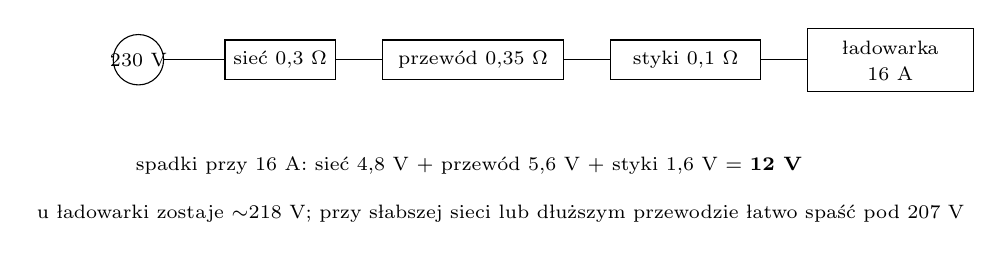
\begin{tikzpicture}[x=1cm,y=1cm,font=\scriptsize]
\draw (0,0.6) circle (0.32); \node at (0,0.6) {230 V};
\draw (0.32,0.6) -- (1.1,0.6);
\draw (1.1,0.35) rectangle (2.5,0.85); \node at (1.8,0.6) {sieć 0,3 \ohm};
\draw (2.5,0.6) -- (3.1,0.6);
\draw (3.1,0.35) rectangle (5.4,0.85); \node at (4.25,0.6) {przewód 0,35 \ohm};
\draw (5.4,0.6) -- (6.0,0.6);
\draw (6.0,0.35) rectangle (7.9,0.85); \node at (6.95,0.6) {styki 0,1 \ohm};
\draw (7.9,0.6) -- (8.5,0.6);
\draw (8.5,0.2) rectangle (10.6,1.0); \node at (9.55,0.75) {ładowarka};
\node at (9.55,0.42) {16 A};
\node[align=left] at (4.2,-0.75) {spadki przy 16 A: sieć 4,8 V $+$ przewód 5,6 V $+$ styki 1,6 V $=$ \textbf{12 V}};
\node[align=left] at (4.6,-1.35) {u ładowarki zostaje $\sim$218 V; przy słabszej sieci lub dłuższym przewodzie łatwo spaść pod 207 V};
\end{tikzpicture}
\caption{Obwód rzeczywisty to łańcuch rezystancji. Przykład: 25 m przewodu 2,5 mm$^2$
(0,35 \ohm{} w obie strony) $+$ typowa impedancja sieci $+$ styki.}
\label{fig:spadek}
\end{figure}

\section{Wady NIEKRYTYCZNE --- wszystko działa, ładowanie nie (rozdział główny)}
\label{sec:niekrytyczne}
To jest sedno przewodnika: wady, z którymi klient mieszka od lat bez żadnych objawów --- bo czajnik,
telewizor i pralka ich nie ujawniają --- a które ładowanie EV ujawnia albo pogarsza aż do usterki.
Dla każdej: mechanizm $\to$ dlaczego AGD działa $\to$ co widzi klient przy EV $\to$ pytania
diagnostyczne $\to$ jak potwierdzić.

\subsection{Zużyte lub tanie gniazdo (osłabione styki) --- klasyk ,,grzania wtyczki''}
\textbf{Mechanizm:} sprężyny gniazda tracą docisk (wiek, wielokrotne wtykanie, wcześniejsze
przegrzania, tani osprzęt). Rezystancja styku rośnie z pojedynczych do setek m\ohm. Przy 16~A:
$P=I^2R=256\cdot0{,}3=77$~W --- małe żelazko zamknięte w puszce w ścianie (rys.~\ref{fig:schuko}).
Ciepło dodatkowo osłabia sprężyny i utlenia styki --- wada się \textbf{samopogłębia}, a po wymianie
samej wtyczki/ładowarki \textbf{wraca}, bo źródłem jest gniazdo.
\textbf{Dlaczego AGD działa:} krótkie pobory nie zdążą nagrzać; 77 W przez 3 minuty czajnika to nic,
przez 6 godzin --- topnienie tworzywa (mięknie od $\sim$110--130\stC).
\textbf{Objawy u klienta:} gorąca/przebarwiona wtyczka lub gniazdo, zapach, ślady nadtopienia,
z czasem błędy temperatury wtyczki (ładowarki AMPERE mierzą temperaturę wtyku i wstrzymują pracę)
albo przerywanie ładowania po godzinie--dwóch (nie od razu!).
\textbf{Pytania:} Czy wtyczka po godzinie ładowania jest gorąca (nie ciepła --- gorąca)? Czy siedzi
w gnieździe luźno? Ile lat ma gniazdo, czy było wymieniane? Czy problem pojawia się \emph{po pewnym
czasie}, a nie od razu? Czy na innym gnieździe (np. w innym budynku) jest tak samo?
\textbf{Potwierdzenie:} oględziny i termowizja gniazda pod obciążeniem; na stanowisku ---
reprodukcja stykiem o podwyższonej rezystancji (symulator: odczep 0,15--0,3~\ohm).

\begin{figure}[h]
\centering
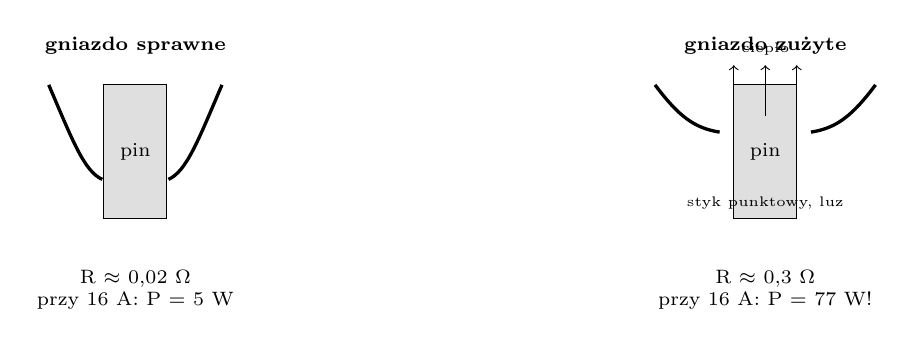
\begin{tikzpicture}[x=1cm,y=1cm,font=\scriptsize]
\foreach \ox/\tit/\r/\p in {0/{gniazdo sprawne}/{R $\approx$ 0,02 \ohm}/{P $=$ 5 W}, 8/{gniazdo zużyte}/{R $\approx$ 0,3 \ohm}/{P $=$ 77 W!}}{
  \node[font=\scriptsize\bfseries] at (\ox+3,2.6) {\tit};
  \draw[fill=gray!25] (\ox+2.6,0.4) rectangle (\ox+3.4,2.1);
  \node at (\ox+3,1.25) {pin};
  \node[align=center] at (\ox+3,-0.5) {\r\\ przy 16 A: \p};}
\draw[very thick] (1.9,2.1) .. controls (2.2,1.4) and (2.35,1.0) .. (2.58,0.9);
\draw[very thick] (4.1,2.1) .. controls (3.8,1.4) and (3.65,1.0) .. (3.42,0.9);
\draw[very thick] (9.6,2.1) .. controls (9.9,1.7) and (10.1,1.55) .. (10.42,1.5);
\draw[very thick] (12.4,2.1) .. controls (12.1,1.7) and (11.9,1.55) .. (11.58,1.5);
\node[font=\tiny] at (11.0,0.6) {styk punktowy, luz};
\foreach \a in {10.6,11.0,11.4}{\draw[->] (\a,1.7) -- (\a,2.35);}
\node[font=\tiny] at (11.0,2.55) {ciepło};
\end{tikzpicture}
\caption{Docisk sprężyn decyduje o rezystancji styku; moc tracona $P=I^2R$ rośnie z kwadratem
prądu i ujawnia się dopiero przy długim, dużym poborze.}
\label{fig:schuko}
\end{figure}

\subsection{Luźny zacisk w puszce lub rozdzielnicy}
\textbf{Mechanizm:} niedokręcony/poluzowany drut w kostce, szybkozłączce, na ,,esce'' --- lokalna
rezystancja jak wyżej, tylko ukryta głębiej. \textbf{AGD działa}, bo grzanie chwilowe.
\textbf{Objawy EV:} przygasanie/miganie światła w rytm ładowania, ciepła ,,eska'' lub puszka,
swąd; czasem restarty ładowarki przy szczycie. \textbf{Pytania:} czy podczas ładowania przygasa
światło w części mieszkania? czy skrzynka/puszka bywa ciepła? czy problem nasila się przy pełnym
prądzie, a znika przy 8--10~A? \textbf{Potwierdzenie:} pomiar spadku napięcia pod obciążeniem
(różnica napięcia gniazdo--rozdzielnica), termowizja rozdzielnicy.

\subsection{Za cienki lub za długi obwód --- spadek napięcia}
\textbf{Mechanizm:} rys.~\ref{fig:spadek}; napięcie u ładowarki maleje proporcjonalnie do prądu.
\textbf{AGD działa:} 210~V zamiast 230~V czajnikowi wydłuża gotowanie o pół minuty --- niezauważalne.
\textbf{Objawy EV:} auto/ładowarka redukuje prąd lub przerywa (próg $\sim$207~V), ładowanie
,,wolniejsze niż ustawione'', przerwy gdy równolegle pracuje bojler/indukcja; latem gorzej (ciepły
przewód ma większą rezystancję), na końcu linii wiejskiej --- dużo gorzej.
\textbf{Pytania:} jak daleko (w metrach kabla) od skrzynki jest gniazdo? garaż/ogród? przedłużacz
(patrz 6.13)? czy problem tylko przy pełnym prądzie / gdy działa coś jeszcze?
\textbf{Potwierdzenie:} pomiar napięcia bez i pod obciążeniem (różnica $>$10~V przy 16~A $=$
obwód słaby); pomiar impedancji pętli.

\subsection{Stara różnicówka typu AC (albo jej brak)}
\textbf{Mechanizm:} rys.~\ref{fig:rcd}. Typ AC nie widzi upływów pulsujących/stałych, a gładki DC
$>$6~mA potrafi ją \textbf{oślepić} także na zwykłe upływy. \textbf{AGD działa:} pralce to nie
przeszkadza --- ona nie generuje gładkiego DC. \textbf{Objawy EV:} dwa przeciwne scenariusze:
(a) RCD-AC \emph{nie wyzwala nigdy} --- pozornie ,,brak problemu'', ale ochrony przy EV realnie
nie ma (wada wychodzi w pomiarach, nie w objawach); (b) starsze egzemplarze --- fałszywe
wyzwolenia od zakłóceń elektroniki auta. \textbf{Pytania:} jaki symbol jest na różnicówce (sama
sinusoida $=$ AC; sinusoida z półfalami $=$ A)? rok instalacji? \textbf{Potwierdzenie:} typ na
aparacie; test RCD miernikiem (prąd i czas zadziałania).

\subsection{Suma upływów wielu urządzeń na wspólnym RCD}
\textbf{Mechanizm:} jeden RCD 30~mA na pół domu; filtry przeciwzakłóceniowe urządzeń dają po
0,5--2~mA legalnego upływu; wilgoć dokłada swoje; ładowarka z autem dokłada 3--6~mA. Suma podchodzi
pod próg --- RCD zgodnie z normą może wyzwolić już od 15~mA. \textbf{AGD działa:} przed EV suma
była niżej progu. \textbf{Objawy EV:} różnicówka pada ,,losowo'', często \textbf{nocą} (wilgoć,
start lodówki) albo dopiero po podłączeniu auta (nie samej ładowarki!); po odłączeniu kilku
sprzętów --- przestaje. \textbf{Pytania:} co jeszcze gaśnie, gdy wyzwala (pół domu czy tylko
ładowarka)? czy pada częściej nocą/po deszczu? czy pada też, gdy auto nie jest wpięte? czy w domu
jest dużo elektroniki/druga lodówka/hydrofor? \textbf{Potwierdzenie:} pomiar prądu upływu
cęgami/RCM na obwodzie; rozwiązanie: dedykowany RCD dla EV.

\subsection{Wątpliwy przewód ochronny PE --- wada z definicji niewidoczna}
\textbf{Mechanizm:} PE przerwany, niedokręcony, skorodowany albo (TN-C) ,,dorobiony'' mostkiem
z N --- na co dzień \emph{żaden} prąd tamtędy nie płynie, więc \emph{nic} tego nie ujawnia.
\textbf{AGD działa} w 100\%. \textbf{Objawy EV:} ładowarka AMPERE sprawdza uziemienie i \textbf{od
razu} zgłasza błąd (ikona złego uziemienia) --- klasyczne zgłoszenie ,,ładowarka wadliwa, bo
wszystko inne działa''; w TN-C z mostkiem za różnicówką --- RCD wyzwala natychmiast przy każdym
starcie. \textbf{Pytania:} czy błąd uziemienia pojawia się od razu po wpięciu (nie po czasie)?
budynek/instalacja sprzed $\sim$1990? czy gniazdo było dokładane samodzielnie? czy w innym budynku
ładowarka działa? \textbf{Potwierdzenie:} pomiar ciągłości PE i pętli L--PE; oględziny gniazda
(mostek N--bolec).

\subsection{Zamieniona L z N w gnieździe}
\textbf{Mechanizm:} po samodzielnej wymianie gniazda przewody trafiają odwrotnie. Dla lampy czy
czajnika bez znaczenia (odbiorniki AC są symetryczne). \textbf{Objawy EV:} ładowarka wykrywa
zamianę i \textbf{blokuje pracę} (deklaracja producenta w instrukcji serii P) --- znowu ,,wszystko
działa, ładowarka nie''. \textbf{Pytania:} czy gniazdo było niedawno wymieniane/dokładane? czy
w innym gnieździe działa? \textbf{Potwierdzenie:} próbnik napięcia; pomiar L--PE (230~V)
i N--PE ($\approx$0~V).

\subsection{Napięcie za wysokie --- sąsiedztwo fotowoltaiki}
\textbf{Mechanizm:} w słoneczne południe falowniki PV w okolicy podnoszą napięcie sieci; przy
słabej sieci lokalnie bywa 250--255~V. \textbf{AGD działa} (znosi to bez protestu).
\textbf{Objawy EV:} auto lub ładowarka odmawia/przerywa \textbf{tylko w słoneczne dni w środku
dnia}, wieczorem i w pochmurne dni --- działa. Bywa mylone z przegrzaniem. \textbf{Pytania:} czy
problem występuje głównie w słoneczne południe, a wieczorem znika? czy klient lub sąsiedzi mają
PV? \textbf{Potwierdzenie:} rejestracja napięcia w ciągu dnia (miernik z zapisem min/max);
u nas --- reprodukcja podwyższonym napięciem (symulator/autotransformator).

\subsection{,,Miękka'' sieć zasilająca (wysoka impedancja przyłącza)}
\textbf{Mechanizm:} długa linia napowietrzna, stary WLZ, koniec wsi --- napięcie mocno siada pod
prądem, choć bez obciążenia jest wzorowe. \textbf{Objawy EV:} jak przy spadku napięcia, ale problem
leży \emph{przed} licznikiem --- wymiana obwodu nic nie da; dodatkowo miga światło w całym domu.
\textbf{Pytania:} czy światło przygasa w \emph{całym} domu przy ładowaniu? jak daleko do
transformatora/jaka zabudowa? \textbf{Potwierdzenie:} pomiar impedancji pętli (duża także L--N),
rejestracja napięcia pod obciążeniem; docelowo zgłoszenie do OSD.

\subsection{Wspólny obwód z innymi odbiornikami}
\textbf{Mechanizm:} ładowarka dzieli ,,eskę'' z lodówką/garażem/hydroforem --- suma prądów
przekracza zabezpieczenie. \textbf{Objawy EV:} B16 wyzwala z opóźnieniem (kwadranse), typowo
\textbf{w nocy}, gdy startuje sprężarka --- rano klient widzi nienaładowane auto i wyłączony obwód.
\textbf{Pytania:} co jeszcze jest na tym samym zabezpieczeniu? wyzwala od razu czy po czasie? czy
pomaga obniżenie prądu w ładowarce? \textbf{Potwierdzenie:} identyfikacja obwodu, pomiar prądu;
rozwiązanie: obwód dedykowany albo niższa nastawa.

\subsection{Aluminiowa instalacja --- usterka, która wraca}
\textbf{Mechanizm:} Al płynie pod śrubą i utlenia się; zacisk dokręcony dziś luzuje się za kilka
miesięcy \emph{sam}. \textbf{AGD:} latami bez objawów. \textbf{Objawy EV:} historia dokładnie jak
w zgłoszeniach serwisowych: grzanie/wyłączanie $\to$ elektryk poprawia $\to$ kilka tygodni OK $\to$
\textbf{wraca}. \textbf{Pytania:} instalacja aluminiowa (budynek 1960--1990 bez wymiany)? czy
usterka już była naprawiana i wróciła? \textbf{Potwierdzenie:} oględziny (szare żyły), termowizja;
rozwiązanie trwałe: wymiana obwodu na Cu / zaciski Al-Cu z pastą.

\subsection{Wilgoć: garaż, gniazdo zewnętrzne, kondensacja}
\textbf{Mechanizm:} wilgoć tworzy ścieżki upływu (mA) w osprzęcie i po izolacji; nocą kondensacja.
\textbf{Objawy EV:} RCD pada po deszczu/nocą; błędy znikają w suche dni. \textbf{Pytania:} gdzie
jest gniazdo (na zewnątrz/garaż nieogrzewany)? korelacja z pogodą? \textbf{Potwierdzenie:} pomiar
rezystancji izolacji obwodu (spada przy wilgoci), pomiar upływu.

\subsection{Przedłużacze i bębny}
\textbf{Mechanizm:} dodatkowa rezystancja styków i przewodu; \textbf{zwinięty bęben grzeje sam
siebie} (dopuszczalny prąd zwiniętego bębna to często 1/4 nominalnego). \textbf{Objawy EV:}
topienie bębna/wtyczek, przerywanie po nagrzaniu. Instrukcja AMPERE wprost zakazuje przedłużaczy.
\textbf{Pytania:} czy ładowarka jest wpięta bezpośrednio? (klienci często nie uznają ,,krótkiego''
przedłużacza za przedłużacz); czy bęben był rozwinięty? \textbf{Potwierdzenie:} wywiad;
reprodukcja na stanowisku z odczepem rezystancji.

\section{Wady krytyczne (krótko --- zwykle widać je nie tylko przy EV)}
\label{sec:krytyczne}
Dla porządku, bo klientom ,,inne rzeczy zwykle działają'', ale trzeba je znać i umieć wychwycić
w rozmowie, bo są niebezpieczne:
\begin{itemize}
\item \textbf{przerwany PEN w TN-C} --- na obudowach pojawia się napięcie z odbiorników; objawy:
,,szczypie'' od pralki/kranu, dziwne napięcia N--PE, migotanie w całym budynku. Natychmiast
elektryk/pogotowie energetyczne;
\item \textbf{brak jakichkolwiek zabezpieczeń różnicowych w łazience/na zewnątrz} przy jednoczesnym
ładowaniu z gniazd zewnętrznych --- ryzyko porażenia;
\item \textbf{,,naprawione'' bezpieczniki (drut w korku), zabezpieczenie za duże względem przewodu}
(np. B25 na 1,5~mm$^2$) --- przewód staje się bezpiecznikiem; przegrzewa się w ścianie;
\item \textbf{uszkodzona izolacja} (wiercenie w ścianie, gryzonie) --- upływy, RCD, w skrajności
zwarcie; przy braku RCD --- pożarowo groźne;
\item \textbf{przeciążone przyłącze/za mała moc umowna} --- główne zabezpieczenie przedlicznikowe
wyzwala przy ładowaniu $+$ kuchnia; to nie wada sprzętu, tylko limit domu (rozwiązanie: niższy
prąd ładowania, DLB, zmiana mocy umownej).
\end{itemize}

\section{Katalog scenariuszy: objaw $\to$ przyczyny $\to$ pytania $\to$ potwierdzenie}
\label{sec:katalog}
Tabela robocza do użycia przy telefonie. Kolejność przyczyn $=$ od najczęstszej. To jest zalążek
katalogu, który stacja testowa będzie rozbudowywać: każdy scenariusz da się \textbf{odtworzyć na
stanowisku} (symulator niedoskonałości instalacji), zapisać zachowanie konkretnego modelu ładowarki
i dopisać do katalogu wpis z twardymi danymi (co pokazuje ekran, po jakim czasie przerywa, co
raportuje aplikacja).

\begin{longtable}{@{}p{0.20\textwidth}p{0.30\textwidth}p{0.44\textwidth}@{}}
\toprule
\textbf{Objaw klienta} & \textbf{Najczęstsze przyczyny} & \textbf{Kluczowe pytania / potwierdzenie}\\
\midrule
grzeje się wtyczka & zużyte gniazdo; przedłużacz/bęben; luźny zacisk za gniazdem; Al & gorąca po
godzinie? luźno siedzi? przedłużacz? wiek gniazda? $\to$ termowizja, wymiana gniazda, obniżenie
prądu do czasu naprawy\\
różnicówka wyzwala & suma upływów na wspólnym RCD; wilgoć; mostek N--PE (TN-C); rzadziej upływ
w aucie/ładowarce & pada od razu czy losowo/nocą? tylko z autem? co jeszcze gaśnie? po deszczu?
$\to$ pomiar upływu, rozdział obwodów; test bez auta\\
błąd uziemienia od razu & wadliwy/brak PE; zamiana L--N; TT ze słabym uziomem & od razu po wpięciu?
budynek sprzed 1990? gniazdo wymieniane samodzielnie? działa w innym budynku? $\to$ pomiar PE/pętli\\
ładuje wolniej niż ustawiono & spadek napięcia (obwód/miękka sieć); auto redukuje; temperatura & ile
metrów od skrzynki? przygasa światło? tylko przy pełnym prądzie? $\to$ pomiar U pod obciążeniem\\
przerywa w środku dnia & za wysokie napięcie (PV); termika latem & słoneczne południe, wieczorem OK?
PV w okolicy? $\to$ rejestracja napięcia\\
przerywa/wybija nocą & wspólny obwód (lodówka); suma upływów $+$ wilgoć & co jest na tym samym
zabezpieczeniu? RCD czy ,,eska'' wybija? $\to$ identyfikacja obwodu\\
działa u nas, u klienta nie & dowolna z powyższych --- środowiskowa & pełny wywiad jak wyżej $\to$
reprodukcja profilu na stanowisku (symulator)\\
naprawione --- zepsuło się znowu & aluminium/luźny zacisk (wada wraca); zużyte gniazdo (źródło poza
ładowarką) & czy naprawiano tylko ładowarkę, a nie instalację? Al? $\to$ skierowanie na naprawę
obwodu, nie sprzętu\\
\bottomrule
\end{longtable}

\section{Słowniczek}
\begin{description}[style=nextline]
\item[L / N / PE / PEN] przewód fazowy / neutralny (roboczy powrót prądu) / ochronny (tylko na
awarię) / połączony N$+$PE w starych sieciach TN-C.
\item[TN-C, TN-C-S, TN-S, TT] układy prowadzenia N i PE --- rozdz.~\ref{sec:uklady}.
\item[RCD (różnicówka) i typy AC/A/F/B] wyłącznik reagujący na prąd uciekający poza obwód;
typ określa, jakie kształty prądu upływu widzi --- rys.~\ref{fig:rcd}.
\item[RDC-DD] układ w ładowarce wykrywający gładki upływ stały $\ge$6~mA (uzupełnia RCD typu A).
\item[Impedancja pętli zwarcia] całkowita ,,oporność'' drogi prądu zwarcia; decyduje, czy
zabezpieczenie wyłączy zwarcie wystarczająco szybko.
\item[Spadek napięcia] obniżenie napięcia na rezystancji przewodów pod prądem; rośnie z prądem
i długością obwodu --- rys.~\ref{fig:spadek}.
\item[WLZ] wewnętrzna linia zasilająca --- odcinek od złącza do rozdzielnicy.
\item[Zerowanie] dawna praktyka łączenia bolca gniazda z przewodem N (TN-C).
\item[Moc umowna] limit mocy w umowie z dostawcą, pilnowany zabezpieczeniem przedlicznikowym.
\end{description}

\section{Podstawy normatywne i źródła}
Seria PN-HD 60364 (instalacje niskiego napięcia; w tym -4-41 ochrona przeciwporażeniowa, -5-52
dobór przewodów, \textbf{-7-722 zasilanie pojazdów elektrycznych}), PN-EN 61008/61009 (RCD),
IEC 61851-1 (interfejs ładowania AC), IEC 62955 (RDC-DD), EN 50160 (parametry napięcia w sieci:
230~V $+10/-10\%$). Materiały w folderze projektu: ,,Przewodnik pomiarów elektrycznych stacji
ładowania'' (W-wa 2024), instrukcja serii P/B AMPERE POINT (deklaracje funkcji kontrolnych),
dokumentacja custom device (symulator niedoskonałości instalacji --- propozycja v3, funkcja
docelowa: budowa niniejszego katalogu scenariuszy). Wartości liczbowe w przykładach są
orientacyjne i służą zrozumieniu zjawisk; dobór konkretnej instalacji zawsze wykonuje elektryk
z uprawnieniami na podstawie pomiarów.

\end{document}
